\subsection{Maximale Drehzahl bei variabler Spannung}\label{subsec:DrehzahlSpanungsabfall}
In diesem Versuch wird das Verhalten des Motors bei Unterspannung untersucht. Dabei wurde der Sollwert für das Drehmoment auf dem Maximum gehalten, während der Motor im Leerlauf dreht. Die Spannung wird dabei langsam erhöht. Die Drehzahl ist dabei elektronisch im Controller auf 3800 RPM begrenzt, da die asynchrone Maschine keine höheren Drehzahlen zulässt und ist in nachfolgender Abbildung \ref{fig:maxDrehzahl} graphisch dargestellt.

\begin{figure}[H]
	\centering
	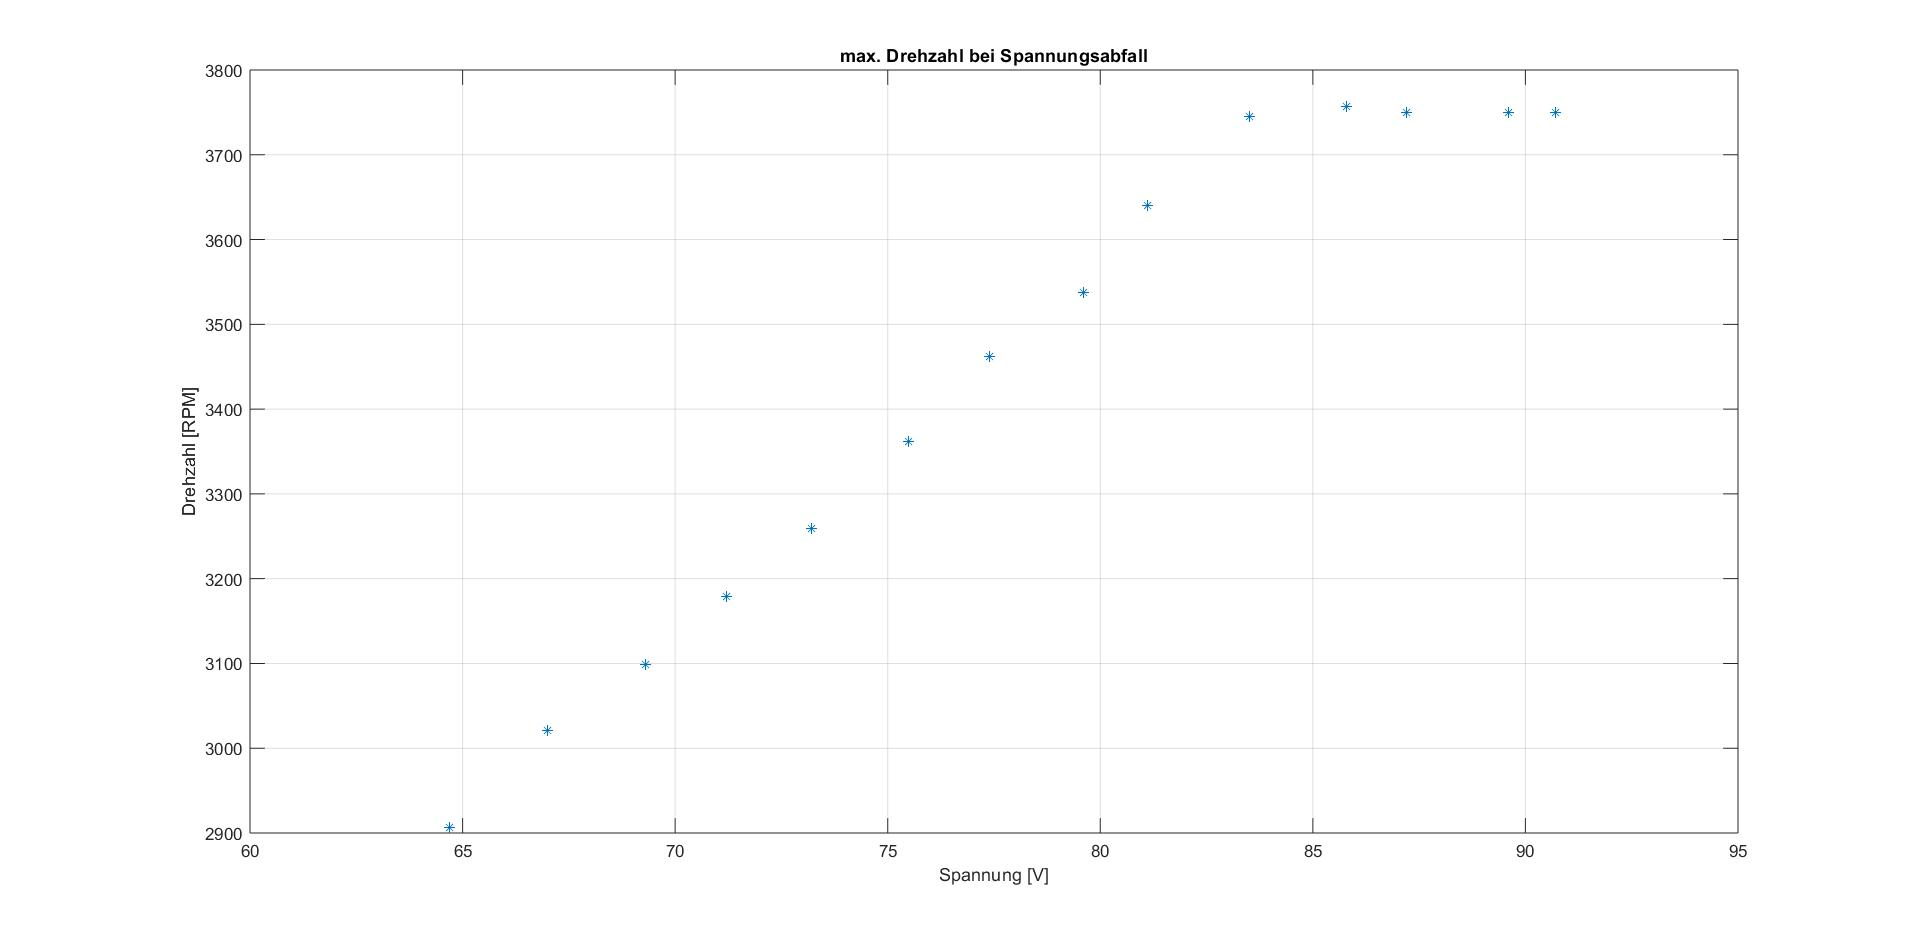
\includegraphics[width=0.8\linewidth]{maxDrehzahl.jpg}
	\caption{Maximale Drehzahl}\label{fig:maxDrehzahl}
\end{figure}

Bei diesem Versuch hat sich gezeigt, dass die Versorgung mindestens 84V bringen muss, damit der BLDC-Motor 3800 RPM erreichen kann. Weiter ist ersichtlich, dass die Leerlaufdrehzahl ca. 45 RPM pro Volt sinkt.

